
This chapter provides an overview of the project in \autoref{sec:overview}, outlines the necessary modifications to the existing project to execute expoSE on the execution platform in \autoref{sec:fwd-z3}, and presents the discovered system-imposed limitations in \autoref{sec:limits}. It then presents the initial idea in \autoref{sec:init-test-plain}. Some of them were contingent upon the platform on which the program was executed. In this case, an Apple MacBook Pro with an M1 Pro chip. 

\section{Overview}
\label{sec:overview}


ExpoSE functions as depicted in \autoref{fig:expose-struc} starting from a component referred to as the distributor to orchestrate the process of symbolic execution. The distributor facilitates the transmission of inputs to the executor, which, as its designation implies, executes the program under test utilizing these inputs. The execution of the program produces a trace, which is subsequently returned to the executor. From this trace, the path condition corresponding to the input is communicated to the SMT Solver. The SMT Solver solves the constraints and then transmits the resulting model back to the executor, enabling the executor to extrapolate alternative inputs. These alternative inputs are subsequently relayed to the distributor, thereby initiating the entire process again. In scenarios where multiple alternative inputs are generated, these inputs are executed concurrently.

For our case, the program under test is not just one script, but consists of both the server and the client, but also of the express model, the request model and the response model. 



\begin{figure}
  \centering
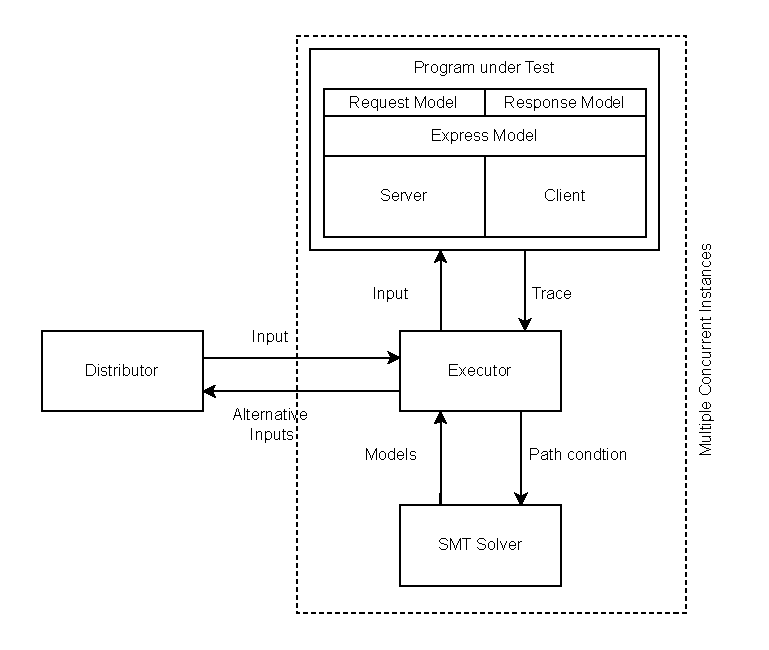
\includegraphics[width=0.7\textwidth]{exposeArchitectureDiagram.pdf}
 \caption[Expose Architecture]{Expose architecture structure, as depicted in \cite{loring_practical_2021}, modified to include the web application with the models for express, request, and response.}
     \label{fig:expose-struc}
\end{figure}


\FloatBarrier
\section{Forwarding Changes of Z3}
\label{sec:fwd-z3}
This section provides a short overview of the changes made to two of the four main parts that make up ExpoSE. Both were relatively simple in nature, but they were required to fix a z3 specific internal error, that kept occurring and caused the execution to fail.

\subsection{Changes to z3}
\label{sec:changes-z3}
As the forked repository of z3 made for expoSE was almost 5 years old, and we occasionally noticed a null pointer exception in the c++ code, we decided to pull the changes from the original repository into the fork, almost 5000 commits, in the hopes of that the null pointer exception has been fixed meanwhile. 
The forwarding went smoothly, with two exceptions. Z3 now includes the type “Char Pointer”, which had to be added to the JavaScript portion (and the Python part, as JavaScript basically copies the bindings from Python) of the binding creation.

The second exception was, that the z3 API now provided a few more callbacks, which, however, required parameters that were not implemented for JavaScript. We have chosen to eliminate these components from our fork over implementing them, as they were not utilized in expoSE and resulted in the failure of the binding generation.

\subsection{Changes to z3JavaScript}
\label{sec:changes-z3js}
With the update to z3 itself, we also had to update the z3JavaScript project, as this defined the types for the JavaScript bindings. It turned out to be a simple issue of adding two new object types (a ParserContextObj and a SimplifierObj) of the type voidp, which is a pointer to the type void.


\section{System-imposed limitations}
\label{sec:limits}
In this section, we will explain the limitations imposed on the application, what it means and how we can circumvent  some of them, while others are a hard  limit.
\subsection{JavaScript Version}
\label{sec:jsversion}
We will start off with the hardest limitation of the application, and that is the fact, that we have to stay in syntax constructs offered by the JavaScript version known as ES6 (or ECMA 2015).

This is a significant limitation, as it implies that we are unable to utilize an essential feature of contemporary JavaScript, specifically \textit{async} and \textit{await}. These two keywords refer to the asynchronous pattern that modern JavaScript employs. Without these, we will not be able to build a modern application, which is a major limitation for a server that might have to wait for resources to load or for a computation-intensive process. For these processes, we now have to rely on callbacks. 



\subsection{HTTP Protocol}
\label{sec:httpprot}
Another limitation we faced was the communication between client and server, as typically, this would happen using HTTP. However, this would mean that we would lose the symbolic state of the program, as the transfer would occur as a byte stream with all data first transformed into a string representation. 
A string, however, cannot be of symbolic type. \\
This means, we had two options:\\
Option A would require us to model the complete HTTP object, with all its bells and whistles, and then include the symbolic state of the program, all while complying with the HTTP standard. This way, we could also test HTTP, and whether the JavaScript implementation works as intended.

Option B is to bypass the transmission of data entirely, by injecting the server into the client, or vice versa, depending on the server structure (more on that later). This would mean that we would have the full symbolic state of the execution, the data would not need to be transformed, and could simply be handed over to the request and response processing on server- and client-side.


We deemed the modelling of the HTTP object out of scope. Therefore, we worked under the assumption, that HTTP works as intended and went for option B, as that meant, we could focus on the actual web application, and could test it in isolation.


\subsection{Symbolic Addresses and Objects}
\label{sec:sym-obj}
While the other limits are specific to our use case, this issue is universal, as pointers can cause a problem on most symbolic execution engines as described by \citet{cha_unleashing_2012}, \citet{coppa_rethinking_2017} and \citet{elkarablieh_precise_2009}, just to name a few. 
Reasoning about the address of a variable poses an issue, as in theory, DSE would have to assume all possible addresses. 
As previously mentioned in \autoref{sec:limits}, \citet{cha_unleashing_2012} proposed a symbolic address, which concretizes writes and only the read is a symbolic operation. 
A similar approach was also taken for ExpoSE, as it concretizes the namespace a variable can occupy, and only its value is resolved symbolically.
ExpoSE initializes a symbolic object by reserving a namespace, concretizing it.


On execution, it then tracks every property access, updating the initial object with a new symbolic variable for the accessed property. 
If we consider this expression:\\
\lstinline[language=JavaScript, gobble=4, escapechar=@]{const object = S$.symbol("object");}
This instruction initilizes the variable object as a new symbolic variable, without any indication that it is an object. 
Should ExpoSE now encounter a property access, i.e.
\lstinline[language=JavaScript, gobble=4, escapechar=@]{if(object.field === "value")},
the property \lstinline{object.field} gets initilized as a new symbolic variable
\lstinline[language=JavaScript, gobble=4, escapechar=@]{object.field = S$.symbol("field");} 
and a path condition gets added, that \lstinline{object} is, in fact, an object.\cite{loring_systematic_2021}

While this works in theory, it is incredibly costly, leading to an explosion of paths, due to the dynamically typed nature of JavaScript, thus adding one path condition per type just on encountering a property access. On black-box testing, where the program has no other option for reasoning what, using completely symbolic objects does increase coverage and helps to find bugs.
In our case, however, where we have full access to the code and where we have knowledge of all input fields, this can be avoided, by creating an object with possible properties already symbolically initialized. This can be done because all unused fields are simply ignored and not adding new path conditions. 
This means, instead of waiting for ExpoSE to find \lstinline{object.field}, we start with an object already containing the field, together with a seed indicating the type, as can be seen in \autoref{lst:sym-obj}.
\begin{minipage}{\linewidth}
    \begin{lstlisting}[language=JavaScript, gobble=4, escapechar=@]
        const object = {
            "field": S$.symbol("field", "string"),
            "numberfield"; S$.symbol("numberfield", 10),
    };
\end{lstlisting}
\captionof{lstlisting}{Concrete object together with symbolic fields initilized.}
\label{lst:sym-obj}
\end{minipage}





\subsection{External Packages}
\label{sec:externalpack}
Our last hard limit was that, even though it was possible to import and use external packages, the DSE engine would assume that any imported package was part of the code. Although technically true, it meant it would be instrumented and create execution branches. This led to a massive explosion in branches, and while it could be used to find bugs and errors in these external packages aswell, it did not offer any use for locating issues in the part of the web application we wanted to test. 
Hence, we opted out of using any external package for now.

\subsection{Dependency Issues}
\label{sec:dep-issues}
While this was not a limit per se, it proved to be an issue with executing the tool chain of expoSE in the first place. When the codebase was created in 2017, almost all personal use computers were made on an x86 platform. While ARM was already widespread in mobile devices, few personal computers were running on an ARM instruction set\footnote{We assume this to be the case, as even the \href{https://www.arm.com/-/media/global/company/investors/Arm\%20Strategic\%20Review\%20-\%202017.pdf?revision=8473a535-6f7e-4ce5-85fe-0eb6f1f75487&la=en}{investor report} in 2017 does not mention them}. Therefore, little to no effort was spent on supporting it. 
With the release of the M1 processor by Apple, this was no longer the case.
This meant that the ARM instruction set went from being rarely supported to a widely spread one.
When we started working on this thesis, we noticed the lack of support. The project required Node version 14, and the package ffi-napi\footnote{https://www.npmjs.com/package/ffi-napi}, that provided the ability to create C bindings, which were used in z3, required Node 16 or higher.
Upgrading the node version initially, would in turn create an error in ffi-napi for the ARM-based M processors~\footnote{As reported in issue https://github.com/node-ffi-napi/node-ffi-napi/issues/248}.\\
While working on this project, the issue got resolved.



\section{Initial Test Plain JS Application}
\label{sec:init-test-plain}
After addressing all the fundamental issues, we began by creating a small server in plain JavaScript to explore whether it is possible to generate requests, process them, and return the correct response for the request. For example, a GET request with the URL '/test' is handled by a GET route registered as '/test', and not incorrectly by the POST route. 

\subsection{Idea}

The objective was to construct a plain JavaScript server by utilizing the http package's method “createServer” and subsequently eliminating all components that depend on http, thus skipping the actual server-client connection.
We had two goals for this: 
\begin{itemize}
    \item  We created a server that had both static and variable routes, notably one route that consisted only of a regular expression, to test whether all routes could be found by the symbolic variable for the path alone.
    \item  We also implemented a short test for injecting code into the response, by asserting that the client cannot send any script tag \lstinline{<script><\script>} in the request data, while asserting that it has to be a valid email. Which in turn meant, expoSE has to try to violate the assertion, by creating inputs, that contain a script tag and are no valid emails. 
\end{itemize}
For the client side we created a bare-bones client, that was generating the symbolic request, and passed it over to the server by calling the onRequest method of the server, which gets called whenever a request is sent, thereby bypassing HTTP. 

\subsection{Evaluation}
This, albeit small test application, showed us, by fulfilling both of our expected outcomes, that it indeed is possible to test a server with expoSE. Finding all the request routes within the server was straightforward, with a minor drawback: the regular expression route was not functional in a switch-case construct due to its use as a literal and not as a regular expression to match a string. 
The second objective was only moderately successful, as, despite demonstrating theoretically that the generation of a string containing a script tag works, it often exceeded the timeout limit, with a few exceptions in a test of 50 runs, where a matching string was immediately generated.

Despite this, we deemed the initial test application a success, as it strongly suggested that it is possible to test a server, explore all possibly routes and locate issues in the validation, data processing and usage of this data. Hence, we moved on from plain JavaScript to the usage of a framework, in our case, Express.js.
